% !TEX encoding = UTF-8
% !TEX program = pdflatex
% !TEX root = MEMOC.tex
% !TEX spellcheck = it-IT

\chapter{Il metodo del simplesso e la dualità}

Inizialmente abbiamo visto come le soluzioni di un problema di programmazione lineare intera si trovino sui vertici della regione ammissibile e come fosse possibile trovare una soluzione in modo grafico.

Con il metodo del simplesso vengono fatte delle considerazioni simili, però a livello algebrico, in modo che possano essere generalizzate a casi che utilizzano più di due variabili.

\section{Le basi del simplesso}

La struttura generale di un modello è:

\begin{align*}
	\min(\max) &f(x) \\
		\st &g_i(x) = b_i \\
			&g_i(x) \leq b_i \\
			&g_i(x) \geq b_i \\
			&x \in \mathbb{R}^n
\end{align*}

\noindent dove $x$ è un vettore colonna di $n$ variabili reali, $f$ è la funzione obiettivo è $g_i$ sono le funzioni che rappresentano i vincoli (sono tutte funzioni $\mathbb{R}^n \to \mathbb{R}$) e i vari $b_i$ sono valori reali.

La cosa chiave è che i valori \textbf{sono numeri reali} e i vincoli sono \textbf{funzioni lineari}.

Si ha quindi che una \textbf{feasible solution} $x \in \mathbb{R}^n$ è un vettore che soddisfa tutti i vincoli, mentre la \textbf{feasible region} è data dall'insieme delle soluzioni feasible e la soluzione ottima è una particolare soluzione feasible che minimizza (o massimizza) la funzione obiettivo.

Il processo di risoluzione consiste quindi nel determinare se:

\begin{itemize}
	\item Il problema è unfeasible.
	\item Il problema è illimitato.
	\item Il problema ha una soluzione ottima.
\end{itemize}

\noindent La regione feasible può essere rappresentata come un \textbf{poliedro}, un'intersezione di un numero finito di semi-spazi chiusi e iperpiani in $\mathbb{R}^n$.

Un problema può quindi essere modellato come:

$$
\min (\max) \{c^T x : x \in P\}
$$

\noindent dove $P$ è un poliedro in $\Rn$.

\begin{figure}[htbp]
	\centering
	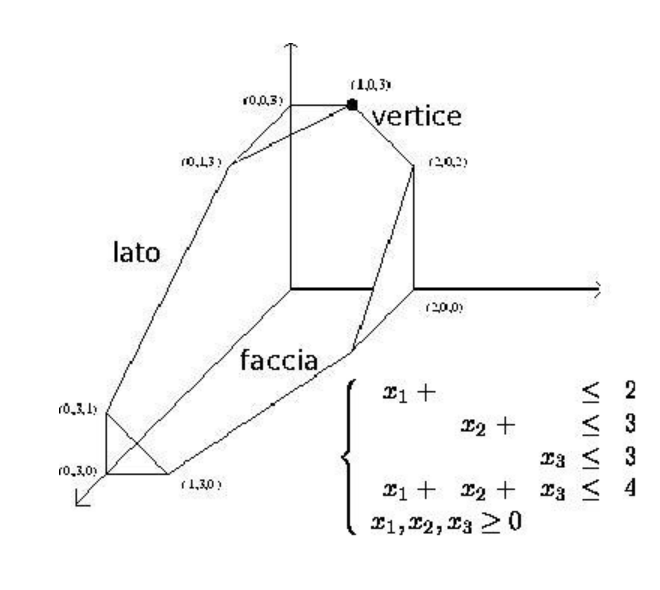
\includegraphics[width=0.6\textwidth]{images/l9-fig-1.png}
\end{figure}

\noindent Un \textbf{vertice} $v \in P$ è un vertice del poliedro $P$ se non è una \textbf{strict convex combination} di due punti distinti di $P$.

Un vertice $z \in \Rn$ è una \textbf{combinazione convessa} di due punti quando

$$
\exists \lambda \in [0,1] : z = \lambda x + (1-\lambda)y
$$

\noindent Viene detta \textbf{strict} se i valori 0 e 1 sono esclusi dall'intervallo.

Una \textbf{combinazione convessa} può essere fatta anche con più di due punti e può essere utilizzata per rappresentare una regione.
$z \in \Rn$ è una combinazione convessa di $x^1, x^2, \ldots, x^k$ se $\exists \lambda_1, \lambda_2, \ldots \lambda_k \geq 0$ tale che 

$$
\sum\limits_{i=1}^{k} \lambda_i = 1 \quad \text{e}\quad z = \sum\limits_{i=1}^{k} \lambda_ix^i
$$

\noindent Per il teorema di \textbf{Minkowski-Weyl}, la combinazione convessa di tutti i vertici di un poliedro permettono di rappresentare tutti i punti che appartengo al poliedro.

Quindi, per il \textbf{teorema del vertice ottimo}, se un problema LP ha può essere rappresentato da un poliedro $P$, allora esiste almeno una soluzione ottima e una di queste è su un vertice.

Questo è un risultato importante perché possiamo limitare la ricerca della soluzione ottima sui vertici di $P$ e non su tutto lo spazio.

\subsection{Rappresentazione algebrica dei vertici}

Considerando tutti i vincoli come delle uguaglianze abbiamo che i vertici del poliedro sono ottenuti intersecando tra loro le rette rappresentate dai vincoli (considerando il caso con due variabili).

Per trasformare i vincoli da disuguaglianze in uguaglianze è necessario aggiungere delle variabili di \textit{slack} che simulano il maggiore o minore.

Ad esempio:

\begin{align*}
3x_1 + 4x_2 &\leq 24 \\
x_1 + 4x_2 &\leq 20 \\
3x_1 + 2x_2 &\leq 18
\end{align*}

\noindent diventa

\begin{align*}
3x_1 + 4x_2 +s_1&= 24 \\
x_1 + 4x_2 +s_2&= 20 \\
3x_1 + 2x_2 +s_3&= 18
\end{align*}

Se si crea un sistema con queste nuove equazioni si ottengono due gradi di libertà, ovvero possiamo porre due variabili qualsiasi a zero per ottenere una soluzione unica.
Ad esempio se $s_1 = s_2=0$, otteniamo un sistema che può essere risolto e la cui soluzione rappresenta il vertice nel quale vengono imposti saturi il primo e secondo vincolo.

\subsection{Forma standard di un problema}

Per rendere l'approccio generico assumiamo che tutti i problemi sono scritti secondo la forma standard:

\begin{align*}
\min &c_1x_1+ c_2x_2 +\ldots + c_nx_n \\
\st &a_{i1}x_1 + a_{i2}x_2 +\ldots+a_{in}x_n = b_i \quad (i = 1 \ldots m) \\
&x_i \in \mathbb{R}_+ \quad (i = 1 \ldots n)
\end{align*}

\noindent Ovvero un problema in quale si minimizza sempre la funzione obiettivo, con tutte le variabili $\geq 0$ (per rendere semplice identificare le soluzioni infeasible), con tutti i vincoli che sono uguaglianze e con tutte le parti destre $b_i$ dei vincoli $\geq 0$.

Si può sempre trasformare un problema generico in forma standard.

\begin{itemize}
	\item Se il problema iniziale è una massimizzazione, basta passare alla minimizzazione e moltiplicare la funzione obiettivo per $-1$.
	\item Se ci sono delle variabili negative è possibile sostituirle con un'altra variabile che è positiva, es $x_+ = - x_-$.
	\item Se ci sono delle disuguaglianze è possibile aggiungere le variabili slack.
	\item Se un $b_i$ è negativo si può moltiplicare tutto il vincolo per $-1$. 
\end{itemize}

\section{Il metodo del simplesso}

\noindent Assumiamo che il problema sia modellato dal sistema $Ax = b$, $A \in \R^{m\times n}, \rho(A) = m, m <n$.

Definiamo come \textbf{base di $A$} una sotto-matrice quadrata $B \in \R^{m \times m }$ tale che abbia rango massimo. 

Abbiamo quindi che $A = [B|N]$ con $det(B) \neq 0$ e $x = \Bigg[ \frac{x_B}{x_N} \Bigg]$ con $x_B \in \R^m$ e $x_N \in \R^{n-m}$.

Così facendo possiamo riscrivere il sistema come 

$$
Ax = b = [B|N]\Bigg[ \frac{x_B}{x_N} \Bigg] = B x_B + N x_N =b
$$

\noindent Posso quindi ricavare i valori di $x_B$, ovvero delle variabili presenti nella base con

$$
x_B = B^{-1}b - B^{-1}N x_N
$$

\noindent Ponendo le variabili $x$ fuori base ($x_N$) uguali a 0, otteniamo una \textbf{soluzione base}.
Il nome \textbf{base} deriva dal fatto che l'insieme dei vettori che compongono la base sono tutti linearmente indipendenti.

Quindi in una soluzione base abbiamo almeno $n-m$ variabili uguali a 0 (se ce ne sono di più la base diventa degenere).

Tornando al nostro problema di partenza abbiamo che una soluzione base diventa \textbf{feasible} quando soddisfa tutti i vincoli di partenza, ovvero

$$
x_B = B^{-1}b \geq 0
$$

\noindent Si ha quindi che i vertici del poliedro sono una feasible basic solution del sistema.

Per ottenere delle basi diverse, e quindi cercare un altro vertice, basta cambiare quali variabili sono fissate a 0.

\begin{figure}[htbp]
	\centering
	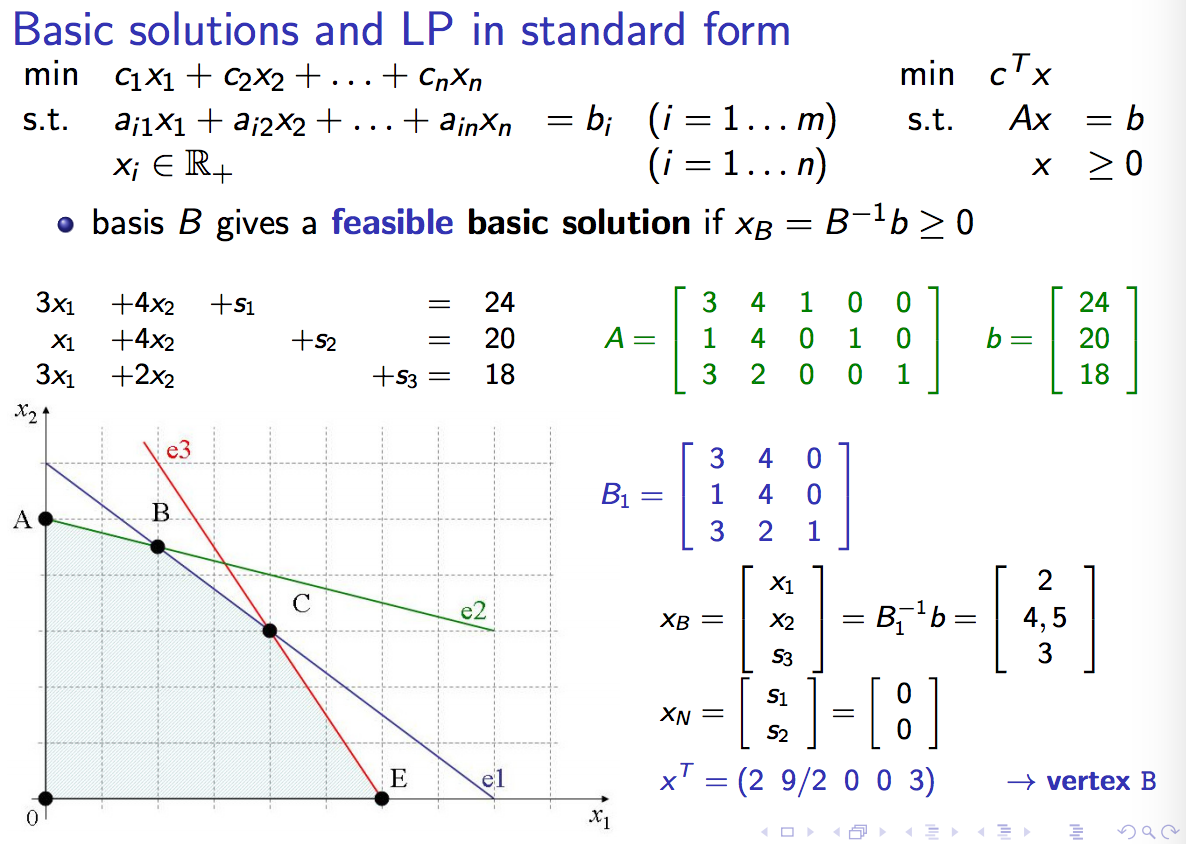
\includegraphics[width=.7\textwidth]{images/l9-fig-2.png}
\end{figure}

\subsection{Algoritmo di massima}

\begin{enumerate}
	\item Trasforma il problema in forma standard.
	\item $incumbent = +\infty$ (soluzione migliore trovata).
	\item Ripeti finché non ci sono altre combinazioni di colonne:
	\begin{itemize}
		\item Genera una combinazione di $m$ colonne di $A$.
		\item Calcola $B$ come la corrispondente sotto-matrice di $A$.
		\item Se il determinante di $B$ è 0, riparti, altrimenti calcola $x_B$.
		\item Se $x_B \geq 0$ e $c^Tx_B \leq incument$, allora aggiorna $incumbent$. 
	\end{itemize}
\end{enumerate}

\noindent Così facendo c'è un'esplosione combinatoria delle soluzioni ed è quindi necessario trovare delle strategie di esplorazione migliori.

Inoltre, la scelta delle colonne da tenere in base può essere a sua volta vista come un problema di ottimizzazione da risolvere con la ricerca locale.
Utilizzando però una strategia di generazione del vicinato che porta ad avere esattamente un vicino, che è una base feasible e che migliora la funzione obiettivo.

Questo viene fatto scrivendo la funzione obiettivo in funzione delle variabili che sono fuori base:

$$
z = c^T x = c_{B}^T x_B + c_{N}^T x_N = c_{B}^T B^{-1}b + (c_{N}^T - c_{B}^T N) x_N
$$

\noindent così facendo si riesce a stimare il miglioramento della funzione obiettivo all'ingresso di una nuova variabile in base e quindi non serve generare il vicinato.

La differenza che c'è quindi tra la soluzione corrente e quella nuova riguarda solamente lo swap tra una variabile in base con una fuori base.
La variabile che esce dalla base deve essere messa a 0 e quindi la variabile che entra in base, entra con un valore tale da rendere la soluzione feasible considerando che l'altra variabile diventa 0.

Per rendere i conti più facile conviene tenere il modello in \textbf{forma canonica} rispetto alla base $B$, ovvero con tutte le variabili in base e la funzione obiettivo espresse sotto forma delle variabili fuori base.

\begin{align*}
	z &= \overline{z}_B + \overline{c}_{N_1} x_{N_1} 
	+ \overline{c}_{N_2} x_{N_2} + \ldots + \overline{c}_{N_{n-m}} x_{N_{n-m}} \\
	x_{B_i} &= \overline{b}_i - \overline{a}_{iN_1} x_{N_1} -\overline{a}_{iN_2} x_{N_2} - \ldots - \overline{a}_{iN_{n-m}} x_{N_{n-m}} \qquad \forall \: i \in [1 \ldots m]
\end{align*}

\noindent dove:

\begin{itemize}
	\item $\overline{z}_B$ è il valore delle funzione obiettivo per la soluzione base.
	\item $\overline{b}_i$ è il valore con il quale la variabile $i$ è in base.
	\item $B_i$ è l'indice dell'$i$-esima variabile in base ($i = 1\ldots m$).
	\item $N_j$ è l'indice della $j$-esima variabile non in base ($j = 1 \ldots n-m$)
	\item $\overline{c}_{N_j}$ è il coefficiente della $j$-esima variabile fuori base nella funzione obiettiva. Prende il nome di \textbf{costo ridotto della variabile rispetto la base $B$}.
	\item $-\overline{a}_{iN_j}$ è il coefficiente della $j$-esima variabile fuori base nel vincolo che rende esplicita la $i$-esima variabile in base.
\end{itemize}

\noindent Il \textbf{costo ridotto} di una variabile rappresenta quanto può incrementare la funzione obiettivo se la variabile alla quale è associato entra in base. I costi ridotti delle variabili in base sono fissi a 0.

Quindi dato un LP e una base feasible $B$, se tutti i costi ridotti rispetto alla base $B$ sono $\geq 0$, allora $B$ è una base ottima.
Non è però detto il contrario, perché possono esserci delle basi ottime che hanno dei costi ridotti negativi.

\subsubsection{Cambio di base}

Data una base feasible $B$, per ottenere una base adiacente, feasible e che migliora la funzione obiettivo è necessario scegliere una colonna (variabile) da far entrare in base e una da far uscire.

Entra in base una qualsiasi variabile $x_h$ che ha il relativo costo ridotto negativo, mentre la variabile che esce viene scelta con la \textbf{min ratio rule}.

Ovvero per le variabili in base vale:

$$
x_{B_i} \geq 0 \Rightarrow b_i - \overline{a}_{ih}x_h \geq 0 \forall \: i \Rightarrow  x_h \leq \frac{\overline{b}_i}{\overline{a}_{ih}} \forall \: i \: : \overline{a}_{ih} > 0.
$$

\noindent scelgo quindi di togliere la variabile

$$
t = \arg \min_{i = 1 \ldots m} \bigg\{ \frac{\overline{b}_i}{\overline{a}_{ih}}  : \overline{a}_{ih} > 0 \bigg\}
$$

\noindent quindi esce dalla base la variabile $x_{B_t}$.

Così facendo, la nuova variabile che entra in base riesce a prendere il valore migliore possibile, mantenendo comunque la soluzione feasible.

C'è da notare che se c'è una certa variabile $x_h$ ha $\overline{c}_h < 0$ e se $a_{ih} \leq 0, \forall i$, si ha che c'è una soluzione feasible anche se $x_h \to +\infty$ e quindi il problema è \textbf{illimitato}, perché posso sempre trovare una soluzione migliore.

\subsection{Algoritmo del simplesso nel dettaglio}

\begin{enumerate}
	\item Trasforma il PL in forma standard e trova una base iniziale feasible $B$. La base può essere trovata risolvendo un problema artificiale.
	\item Ripeti finché non trovi una soluzione ottima o non ti accorgi che il problema è illimitato:
	\begin{itemize}
		\item Poni il problema in forma canonica rispetto la base $B$
		\begin{align*}
		z &= \overline{z}_B + \overline{c}_{N_1} x_{N_1} 
		+ \overline{c}_{N_2} x_{N_2} + \ldots + \overline{c}_{N_{n-m}} x_{N_{n-m}} \\
		x_{B_i} &= \overline{b}_i - \overline{a}_{iN_1} x_{N_1} - \overline{a}_{iN_2} x_{N_2} - \ldots - \overline{a}_{iN_{n-m}} x_{N_{n-m}} \qquad \forall \: i \in [1 \ldots m]
		\end{align*}
		\item Se $\overleftarrow{c}_j \geq 0 \forall \ j$, la base $B$ è ottima. Fermati.
		\item Se $\exists h : \overline{c}_h < 0 , \overline{a}_{ih}\leq 0 \ \forall i$, il problema è illimitato. Fermati.
		\item Scegli una variabile $x_h$ da portare in base tra tutte quelle con costi ridotti negativi.
		\item Trova la variabile $x_{B_t}$ con $ t = \arg \min_{i = 1 \ldots m} \bigg\{ \frac{\overline{b}_i}{\overline{a}_{ih}}  : \overline{a}_{ih} > 0 \bigg\}$
		\item $B \leftarrow B \oplus A_h \ominus A_{B_t}$, ovvero effettua il cambio di base.
	\end{itemize}
\end{enumerate}

\noindent A livello pratico è possibile raggruppare il tutto in un'unica matrice rappresentante la forma canonica del problema che prende il nome di \textbf{tableau del simplesso}.
Così facendo è possibile modellare le operazioni di cambio base utilizzando Gauss-Jordan, fino a che non viene trovata una base ottima oppure ci si accorge che il problema è illimitato.

\begin{figure}[htbp]
	\centering
	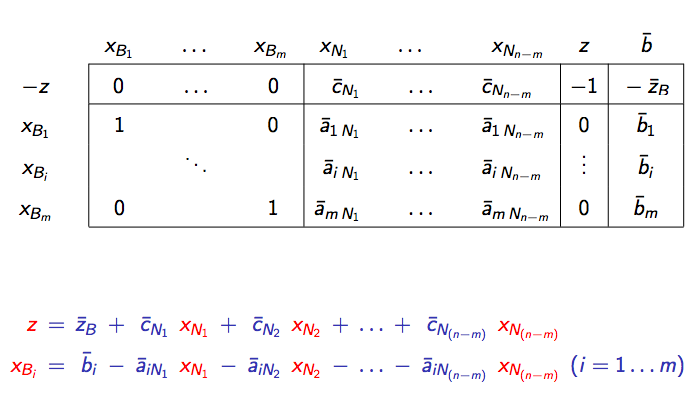
\includegraphics[width = .7\textwidth]{images/l9-fig-3.png}
	\caption{Il talbeau del simplesso}
\end{figure}










